% Generated LaTeX file for compound CID: 80046
\documentclass[tikz]{standalone}
\definecolor{274A4A}{HTML}{274A4A}
\definecolor{D5D500}{HTML}{D5D500}
\begin{document}
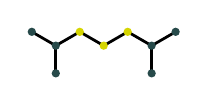
\begin{tikzpicture}[x=1pt,y=1pt]
  \draw[line width=1pt] (54.64,7.50) -- (45.98,2.50);
  \draw[line width=1pt] (54.64,7.50) -- (63.30,2.50);
  \draw[line width=1pt] (37.32,7.50) -- (45.98,2.50);
  \draw[line width=1pt] (37.32,7.50) -- (28.66,2.50);
  \draw[line width=1pt] (63.30,2.50) -- (71.96,7.50);
  \draw[line width=1pt] (63.30,2.50) -- (63.30,-7.50);
  \draw[line width=1pt] (28.66,2.50) -- (20.00,7.50);
  \draw[line width=1pt] (28.66,2.50) -- (28.66,-7.50);
  \filldraw[fill=D5D500, draw=none] (54.64,7.50) circle (1.5pt);
  \filldraw[fill=D5D500, draw=none] (37.32,7.50) circle (1.5pt);
  \filldraw[fill=D5D500, draw=none] (45.98,2.50) circle (1.5pt);
  \filldraw[fill=274A4A, draw=none] (63.30,2.50) circle (1.5pt);
  \filldraw[fill=274A4A, draw=none] (28.66,2.50) circle (1.5pt);
  \filldraw[fill=274A4A, draw=none] (71.96,7.50) circle (1.5pt);
  \filldraw[fill=274A4A, draw=none] (63.30,-7.50) circle (1.5pt);
  \filldraw[fill=274A4A, draw=none] (20.00,7.50) circle (1.5pt);
  \filldraw[fill=274A4A, draw=none] (28.66,-7.50) circle (1.5pt);
\end{tikzpicture}
\end{document}